\documentclass[border=10pt]{standalone}
\usepackage[svgnames]{xcolor}
\usepackage{amsmath}
\usepackage{pgfplots}
\pgfplotsset{compat=newest}
\usepackage[sfdefault]{FiraSans}
\usepackage{FiraMono}
\renewcommand*\familydefault{\sfdefault}
\begin{document}
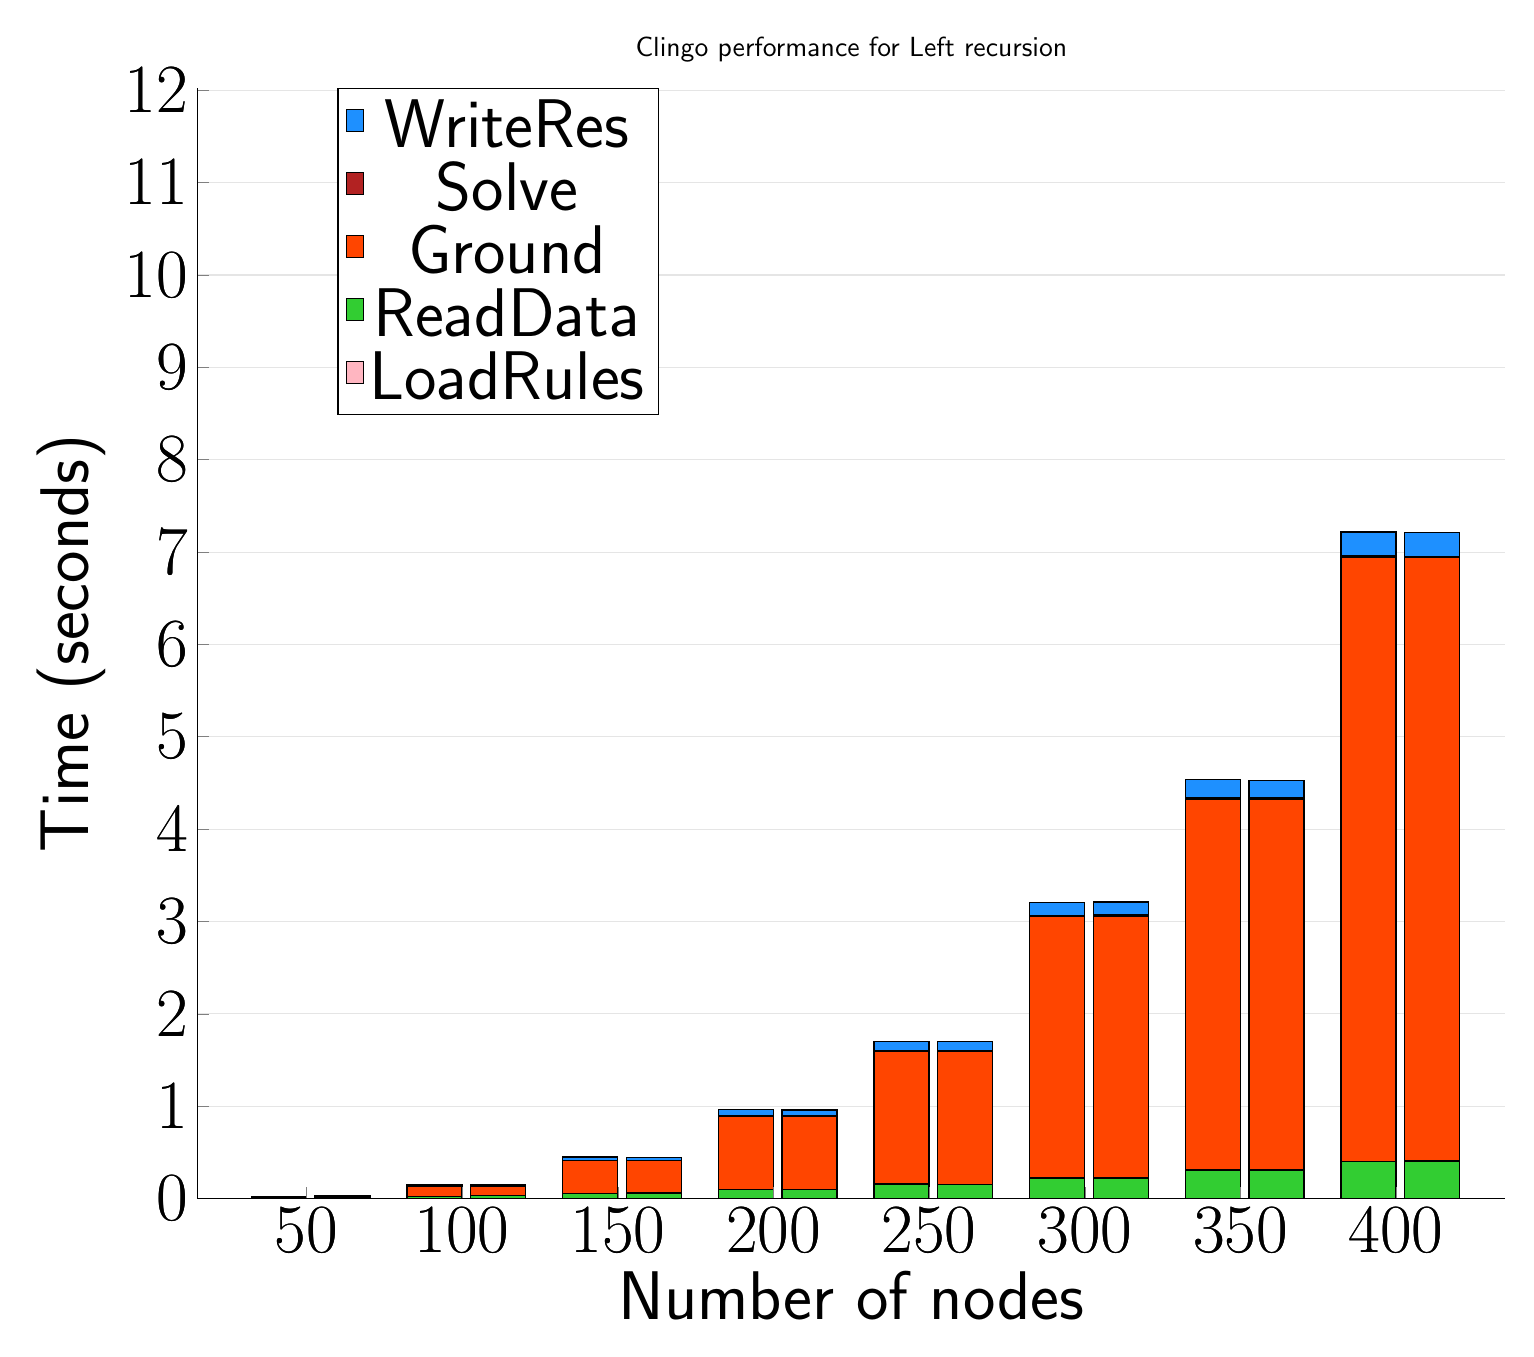
\begin{tikzpicture}
\begin{axis}[
   ybar stacked,
   title={Clingo performance for Left recursion},
   bar shift=-10pt,
   width=1.5\textwidth,
   bar width=0.7cm,
   ymajorgrids, tick align=inside,
   major grid style={draw=gray!20},
   xtick=data,
   ymin=0, ymax=12.025999999046325,
   axis x line*=bottom,
   axis y line*=left,
   enlarge x limits=0.1,
   legend style={
       at={(0.23, 1)},
       anchor=north,
       legend columns=1,
       font=\Huge,
   },
   ylabel={Time (seconds)},
   xlabel={Number of nodes},
   label style={font=\Huge},
   tick label style={font=\Huge},
]
\addlegendimage{fill=DodgerBlue, draw=black, line width=0.2pt}
\addlegendentry{WriteRes}
\addlegendimage{fill=FireBrick, draw=black, line width=0.2pt}
\addlegendentry{Solve}
\addlegendimage{fill=OrangeRed, draw=black, line width=0.2pt}
\addlegendentry{Ground}
\addlegendimage{fill=LimeGreen, draw=black, line width=0.2pt}
\addlegendentry{ReadData}
\addlegendimage{fill=LightPink, draw=black, line width=0.2pt}
\addlegendentry{LoadRules}
\addplot +[fill=LightPink, draw=black, line width=0.5pt] coordinates {
    (50, 0.0)
    (100, 0.0)
    (150, 0.0)
    (200, 0.0)
    (250, 0.0)
    (300, 0.0)
    (350, 0.0)
    (400, 0.0)
};
\addplot +[fill=LimeGreen, draw=black, line width=0.5pt] coordinates {
    (50, 0.005999994277954101)
    (100, 0.02500002384185791)
    (150, 0.0549999475479126)
    (200, 0.09900000095367431)
    (250, 0.15699992179870606)
    (300, 0.22200000286102295)
    (350, 0.3100000858306885)
    (400, 0.40099995136260985)
};
\addplot +[fill=OrangeRed, draw=black, line width=0.5pt] coordinates {
    (50, 0.016000032424926758)
    (100, 0.10599997043609619)
    (150, 0.35700011253356934)
    (200, 0.7960000276565552)
    (250, 1.4390000104904175)
    (300, 2.8359999656677246)
    (350, 4.015999960899353)
    (400, 6.5440000057220455)
};
\addplot +[fill=FireBrick, draw=black, line width=0.5pt] coordinates {
    (50, 0.0)
    (100, 0.0)
    (150, 0.0019999980926513673)
    (200, 0.0029999971389770507)
    (250, 0.005999994277954101)
    (300, 0.009999990463256836)
    (350, 0.011999988555908203)
    (400, 0.016000008583068846)
};
\addplot +[fill=DodgerBlue, draw=black, line width=0.5pt] coordinates {
    (50, 0.003000020980834961)
    (100, 0.016000032424926758)
    (150, 0.03399999141693115)
    (200, 0.06500000953674316)
    (250, 0.10000007152557373)
    (300, 0.14000000953674316)
    (350, 0.19700005054473876)
    (400, 0.2559999942779541)
};
\end{axis}
\begin{axis}[
   ybar stacked,
   bar shift=13pt,
   width=1.5\textwidth,
   bar width=0.7cm,
   ymajorgrids, tick align=inside,
   major grid style={draw=none},
   xtick=data,
   ymin=0, ymax=12.025999999046325,
   axis x line*=none,
   axis y line*=none,
   enlarge x limits=0.1,
   label style={font=\Huge},
   tick label style={font=\Huge},
]
\addplot +[fill=LightPink, draw=black, line width=0.5pt] coordinates {
    (50, 0.0)
    (100, 0.0)
    (150, 0.0)
    (200, 0.0)
    (250, 0.0)
    (300, 0.0)
    (350, 0.0)
    (400, 0.0)
};
\addplot +[fill=LimeGreen, draw=black, line width=0.5pt] coordinates {
    (50, 0.009999999999999997)
    (100, 0.030000000000000006)
    (150, 0.06000000000000001)
    (200, 0.09999999999999999)
    (250, 0.154)
    (300, 0.22200000000000003)
    (350, 0.30799999999999994)
    (400, 0.4069999999999999)
};
\addplot +[fill=OrangeRed, draw=black, line width=0.5pt] coordinates {
    (50, 0.010000000000000004)
    (100, 0.09899999999999999)
    (150, 0.35000000000000003)
    (200, 0.792)
    (250, 1.4369999999999998)
    (300, 2.8369999999999997)
    (350, 4.015)
    (400, 6.531000000000001)
};
\addplot +[fill=FireBrick, draw=black, line width=0.5pt] coordinates {
    (50, 0.0)
    (100, 0.000999999999999998)
    (150, 0.0020000000000000018)
    (200, 0.003999999999999992)
    (250, 0.007000000000000006)
    (300, 0.010000000000000054)
    (350, 0.013000000000000168)
    (400, 0.014999999999999947)
};
\addplot +[fill=DodgerBlue, draw=black, line width=0.5pt] coordinates {
    (50, 0.010000000000000004)
    (100, 0.01800000000000002)
    (150, 0.03499999999999998)
    (200, 0.061999999999999965)
    (250, 0.10100000000000002)
    (300, 0.14099999999999993)
    (350, 0.19199999999999964)
    (400, 0.257)
};
\end{axis}
\end{tikzpicture}

\end{document}
